\section{Finger Knuckle Recognition}

As for the dataset, it can offer a total of 120 subjects that included images from Indian, Chinese and European subjects. Each subject provided a total of 30 images which included multiple fingerprint and finger knuckle images.
However, there are multiple individuals (048,049,050...) whose samples were taken in very dark ambient light, and in turn, the finger knuckle texture is not clear as shown on the Fig. \ref{dark-subjects}. In this special case, the YOLOv5x-CSL model hardly detect the finger knuckle from these dark images. Therefore, as for these unclear subjects, I used the segmented finger knuckle which is offered by the dataset (segmented by Mask R-CNN).

\begin{figure}[h]
    \centering
    \subfloat[]{
        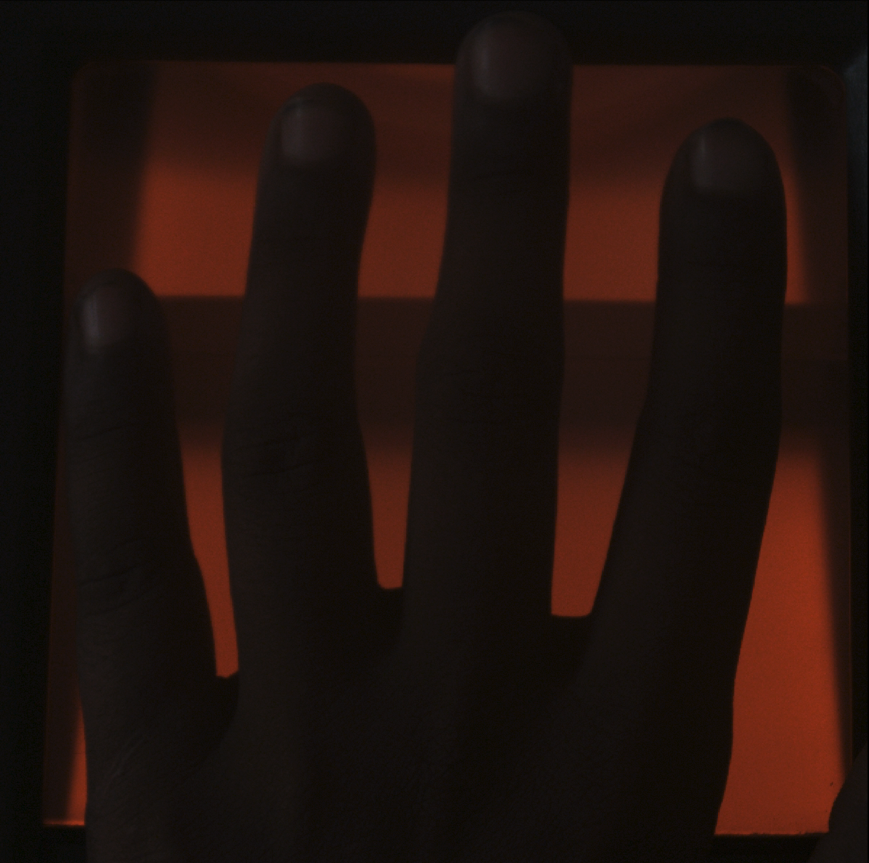
\includegraphics[width=1.2in]{Figure/09-09-2022/1.png}
        \label{}}
    \subfloat[]{
        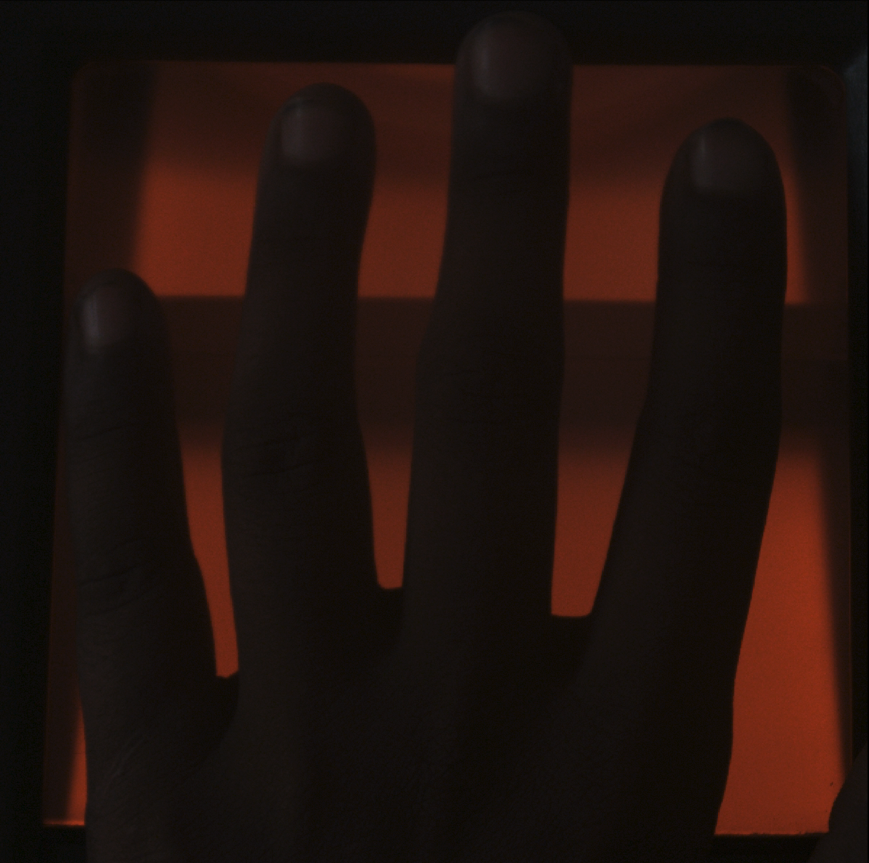
\includegraphics[width=1.2in]{Figure/09-09-2022/1.png}
        \label{}}
    \subfloat[]{
        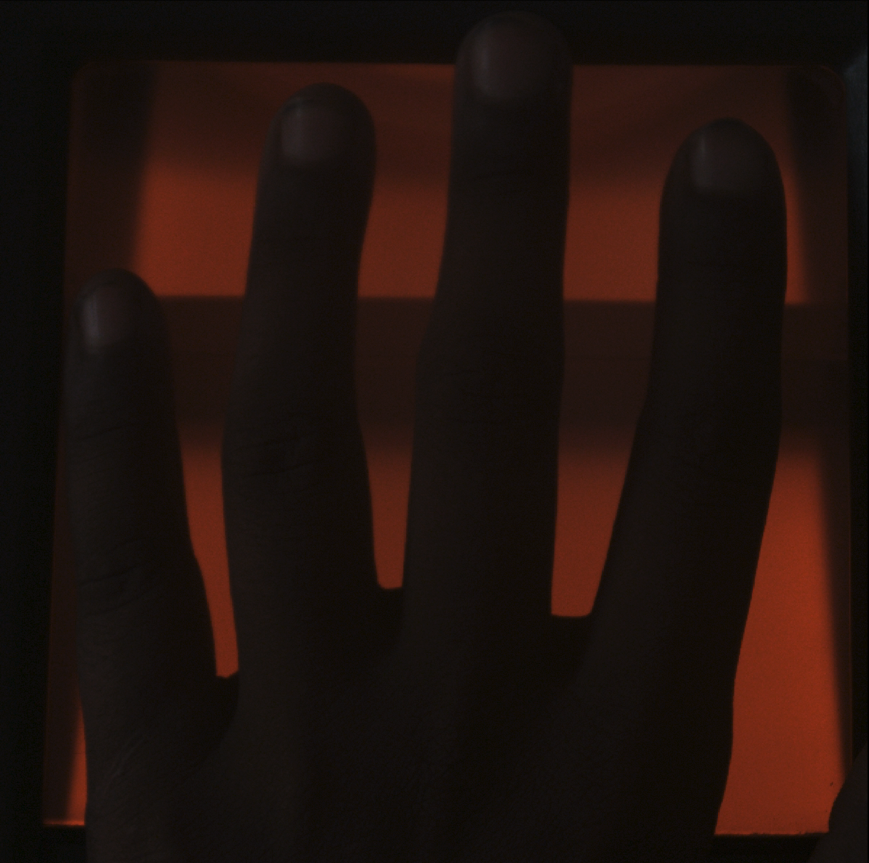
\includegraphics[width=1.2in]{Figure/09-09-2022/1.png}
        \label{}}
    \subfloat[]{
        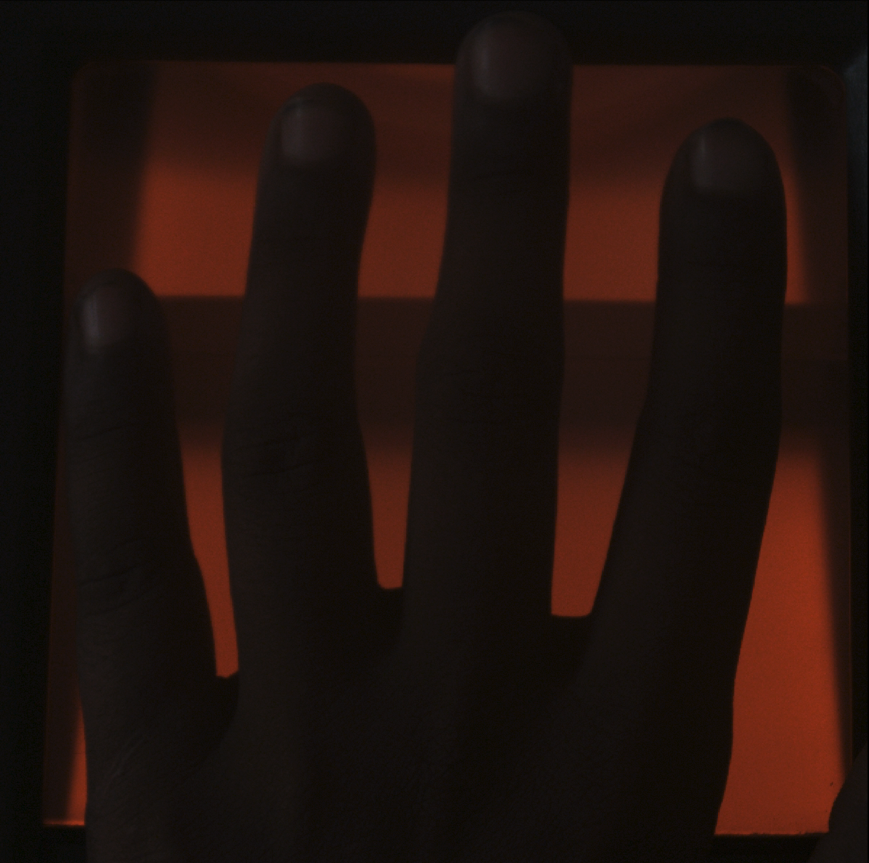
\includegraphics[width=1.2in]{Figure/09-09-2022/1.png}
        \label{}}
    \subfloat[]{
        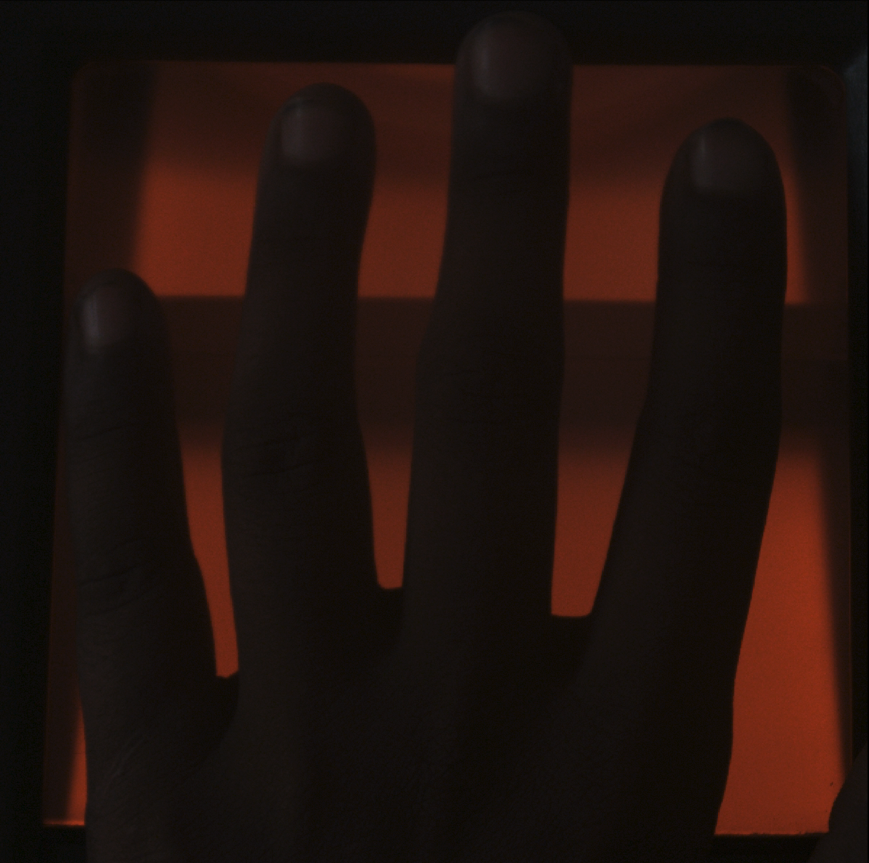
\includegraphics[width=1.2in]{Figure/09-09-2022/1.png}
        \label{}}

    \caption{Show some examples that are captured under dark illumination.}
    \label{dark-subjects}
\end{figure}

The quality of segmented finger knuckle by Mask R-CNN (offered on the dataset) is lower than segmented finger knuckle by YOLOv5x-CSL model. Although it uses the angle of finger to normalize the finger knuckle, the angle is not accurate than YOLOv5x-CSL. When I was labeling the ground truth, I chose the angle of the vertical majority finger knuckle texture as the finger knuckle angle. Secondly, the center of the bounding box is not the center of finger knuckle on the segmented finger knuckle on the dataset.

\begin{figure}[h]
    \centering
    \subfloat[]{
        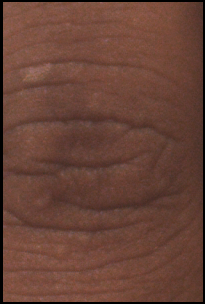
\includegraphics[width=0.6in]{Figure/09-09-2022/dataset-01.png}
        \label{}}
    \subfloat[]{
        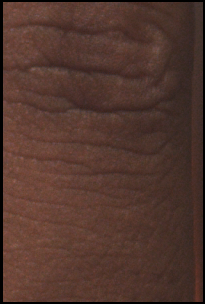
\includegraphics[width=0.6in]{Figure/09-09-2022/dataset-02.png}
        \label{}}
    \subfloat[]{
        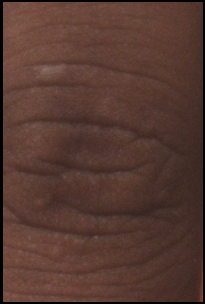
\includegraphics[width=0.6in]{Figure/09-09-2022/dataset-03.png}
        \label{}}
    \subfloat[]{
        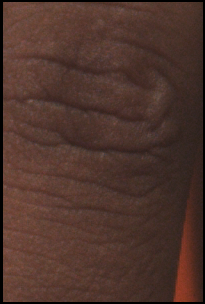
\includegraphics[width=0.6in]{Figure/09-09-2022/dataset-04.png}
        \label{}}
    \subfloat[]{
        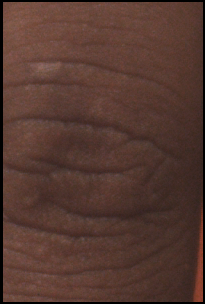
\includegraphics[width=0.6in]{Figure/09-09-2022/dataset-05.png}
        \label{}}
    \subfloat[]{
        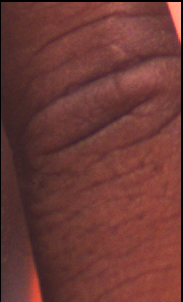
\includegraphics[width=0.6in]{Figure/09-09-2022/dataset-1.png}
        \label{}}
    \subfloat[]{
        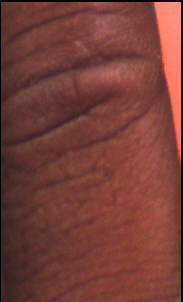
\includegraphics[width=0.6in]{Figure/09-09-2022/dataset-2.png}
        \label{}}
    \subfloat[]{
        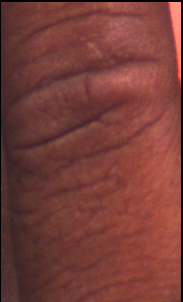
\includegraphics[width=0.6in]{Figure/09-09-2022/dataset-3.png}
        \label{}}
    \subfloat[]{
        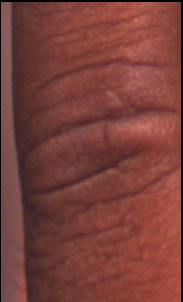
\includegraphics[width=0.6in]{Figure/09-09-2022/dataset-4.png}
        \label{}}
    \subfloat[]{
        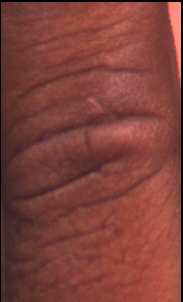
\includegraphics[width=0.6in]{Figure/09-09-2022/dataset-5.png}
        \label{}}

    \subfloat[]{
        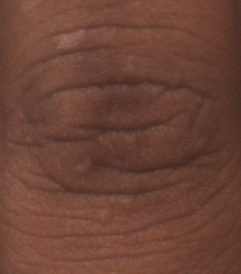
\includegraphics[width=0.6in]{Figure/09-09-2022/yolov5-01.jpg}
        \label{}}
    \subfloat[]{
        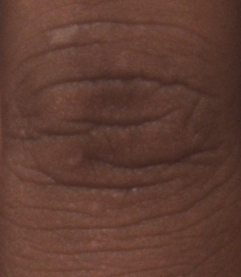
\includegraphics[width=0.6in]{Figure/09-09-2022/yolov5-02.jpg}
        \label{}}
    \subfloat[]{
        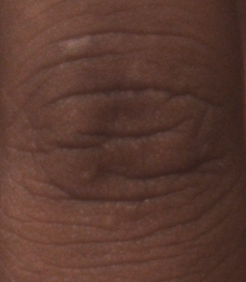
\includegraphics[width=0.6in]{Figure/09-09-2022/yolov5-03.jpg}
        \label{}}
    \subfloat[]{
        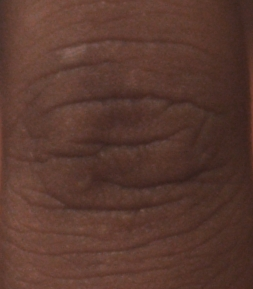
\includegraphics[width=0.6in]{Figure/09-09-2022/yolov5-04.jpg}
        \label{}}
    \subfloat[]{
        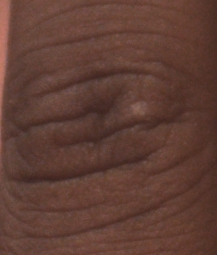
\includegraphics[width=0.6in]{Figure/09-09-2022/yolov5-05.jpg}
        \label{}}
    \subfloat[]{
        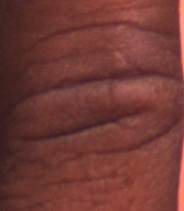
\includegraphics[width=0.6in]{Figure/09-09-2022/yolov5-1.jpg}
        \label{}}
    \subfloat[]{
        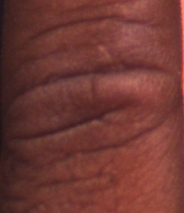
\includegraphics[width=0.6in]{Figure/09-09-2022/yolov5-2.jpg}
        \label{}}
    \subfloat[]{
        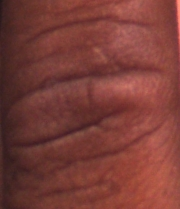
\includegraphics[width=0.6in]{Figure/09-09-2022/yolov5-3.jpg}
        \label{}}
    \subfloat[]{
        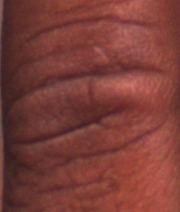
\includegraphics[width=0.6in]{Figure/09-09-2022/yolov5-4.jpg}
        \label{}}
    \subfloat[]{
        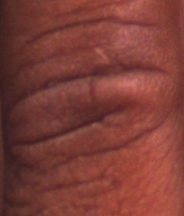
\includegraphics[width=0.6in]{Figure/09-09-2022/yolov5-5.jpg}
        \label{}}

    \caption{The results of the segmentation of the major finger knuckle of two individuals are listed. The first row shows the results using Mask R-CNN and the second row shows the results using YOLOv5x.}
    \label{segmentation}
\end{figure}


\subsection{Matching Performance}
This dataset can provide finger data for both the left and right hand so that the same individual can provide 10 different finger knuckle.We employed more challenging matching protocol to ensure more reliable estimation on the performance from the two biometric images. Therefore, each of the fingers generated 1200 (120×10) genuine and 357000 (120×5×5×119) impostor match scores, for each of the fingerprint and finger knuckle images, and were used to ascertain the performance. Fig. \ref{tech-report} shows the matching accuracy using different finger knuckle from the Tech-Report.
\begin{figure}[h]
    \centering
    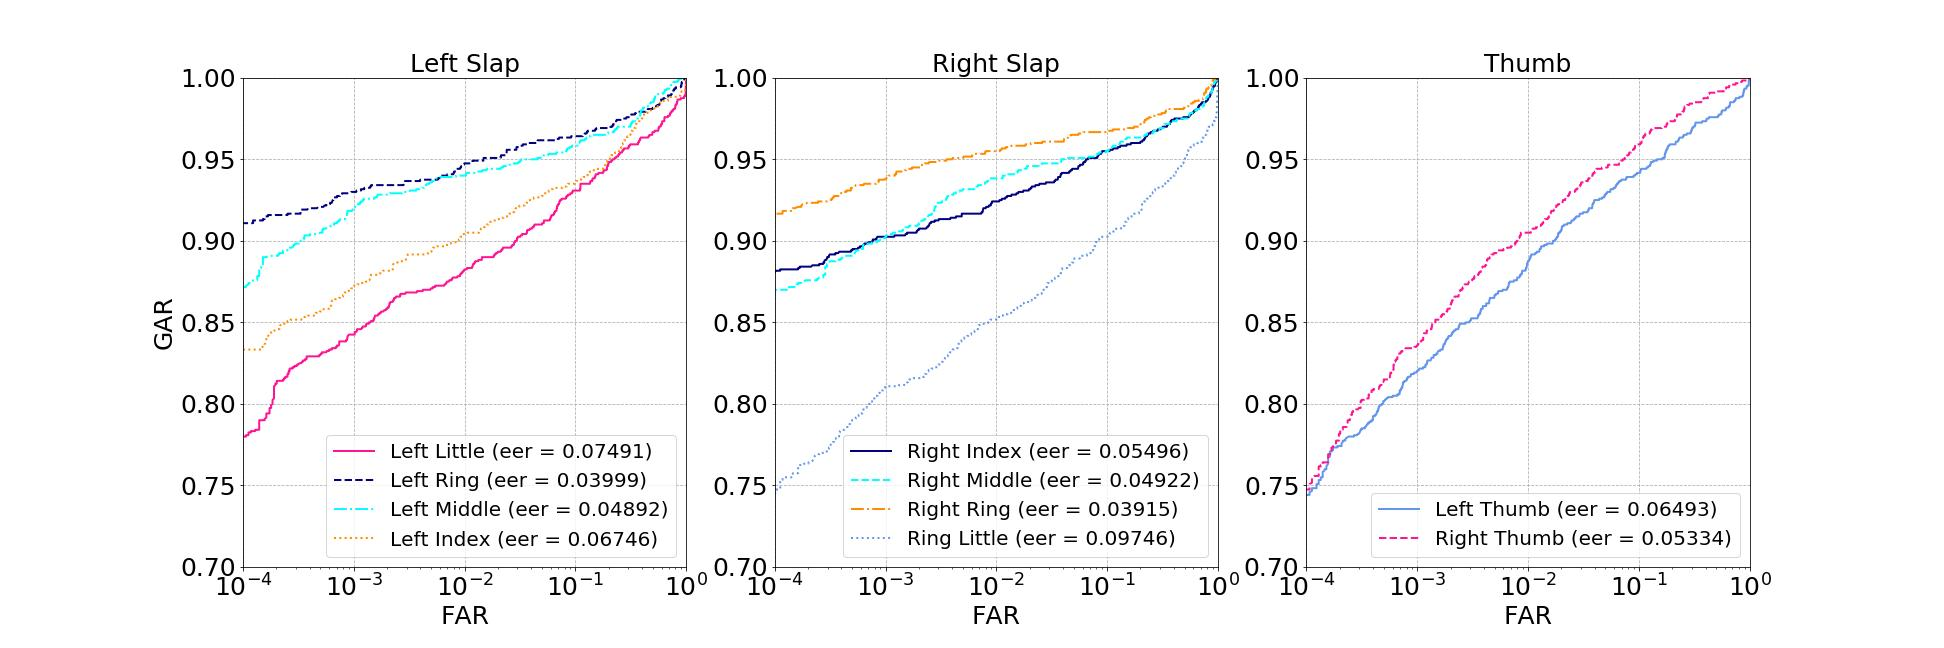
\includegraphics[width=7in]{Figure/09-09-2022/peformance.jpg}
    \caption{Performance from the simultaneously acquired finger knuckle images from left hand, right hand, and thumbs.}
    \label{tech-report}
\end{figure}
\begin{figure}[h]
    \centering
    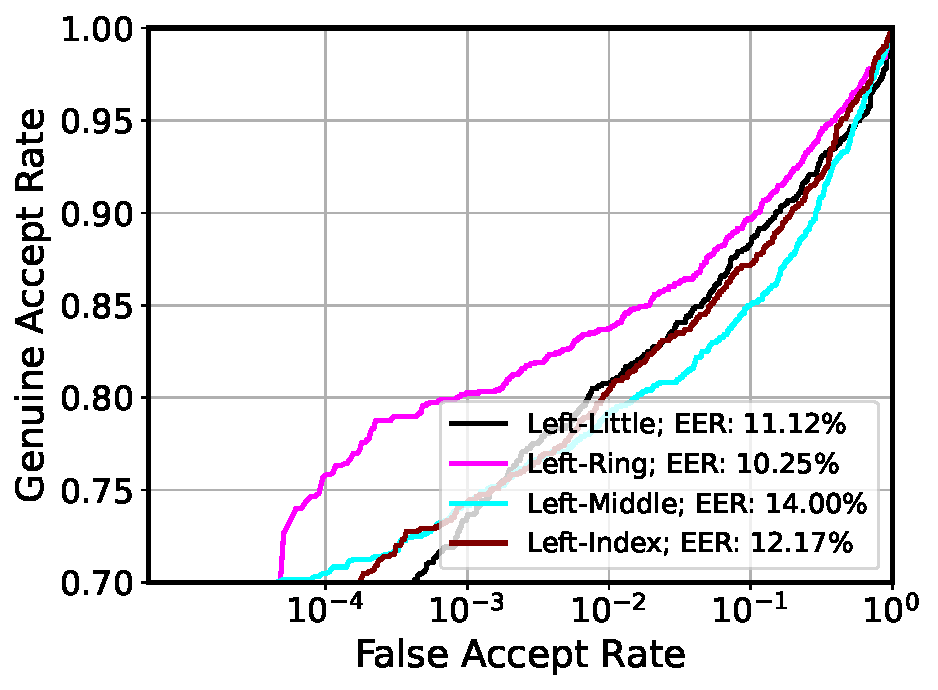
\includegraphics[width=3in]{Figure/09-09-2022/left-roc.pdf}
    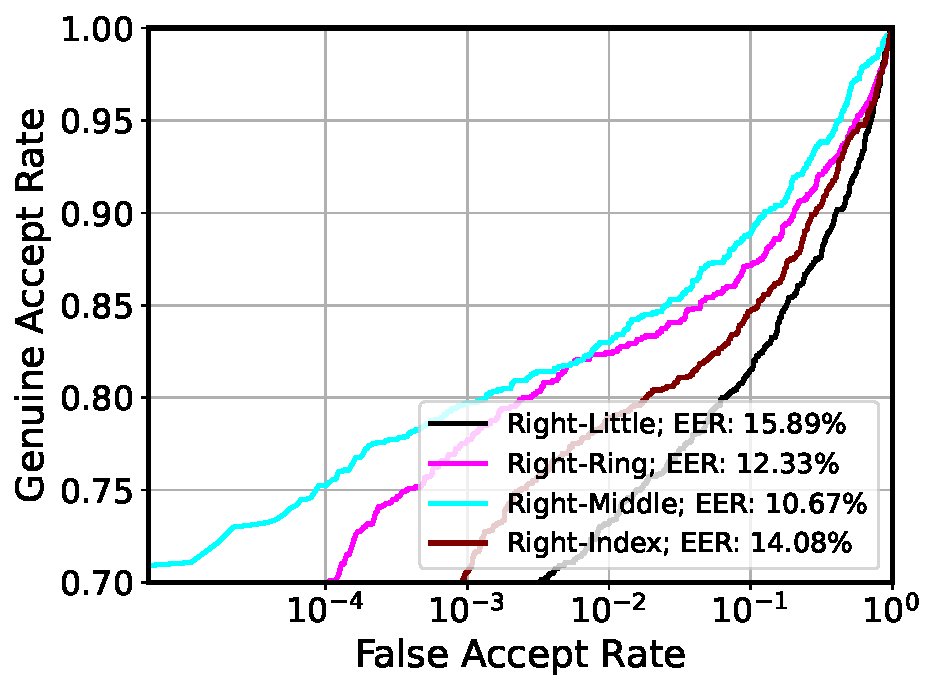
\includegraphics[width=3in]{Figure/09-09-2022/right-roc.pdf}
    \caption{Comparative ROC curve from using little knuckle, ring finger knuckle, middle finger knuckle, and index finger knuckle}
    \label{rfn}
\end{figure}

I also used the RFNet model that has been trained on the finger knuckle v3.0 (deformable) dataset to perform cross database testing on this dataset. And it is the finger knuckle data segmented using the YOLOv5x-CSL model. The corresponding matching accuracy is shown in the Fig. \ref{rfn}, and this result is generally not very accurate, all of them are below 10\% EER.


